% LaTeX body content for Part II, Chapters 7-9
% Research Companion Guide - CNN Strong Gravitational Lens Finding
% Audience: high school student who led the research

\part{What We Did}

\section{Chapter 7: Our Data and Model}

This chapter describes the ingredients we used to train our CNN lens finder: the images, the labels, and the training procedure. Understanding these choices is essential for interpreting the results we present later.

\subsection{The Training Set: 451,681 Cutouts}

We trained our CNN on a large set of small square images called \textbf{cutouts}. Each cutout is a 101$\times$101 pixel region of the sky centered on a galaxy. In total, we had 451,681 cutouts, divided into:
\begin{itemize}
    \item \textbf{316,100} for training (the data the model learns from)
    \item \textbf{135,581} for validation (the data we use to check how well the model generalizes, without ever training on it)
\end{itemize}
The validation set lets us measure performance honestly---if we evaluated on the training data, the model might have ``memorized'' specific examples rather than learned general lens-finding rules.

\subsection{Positive Examples: Tier-A and Tier-B Lenses}

Our positive examples---images that show a strong lens---come in two tiers based on how certain we are that they are real lenses.

\subsubsection{Tier-A Positives: Spectroscopically Confirmed}

\textbf{Tier-A} lenses are the gold standard. We have 277 in training and 112 in validation (389 total). These are \textbf{spectroscopically confirmed} strong lenses.

\textbf{What does ``spectroscopically confirmed'' mean?} When astronomers want to prove that a lens is real, they measure the \textbf{redshift} of the light from different parts of the image. Redshift is a measure of how much the light has been stretched by the expansion of the universe---objects farther away have higher redshift. A strong lens produces multiple images of the same background galaxy. When you split the light from each image into a \textbf{spectrum} (a rainbow showing how much light arrives at each wavelength), you can measure the redshift. If you find \emph{two different redshifts} at the same position on the sky---one from the foreground lens galaxy and one from the background source---you have proof that lensing is occurring. The lens galaxy is in front, bending light from the more distant source. That is spectroscopic confirmation.

Tier-A lenses are our most reliable labels. We use them for our headline recall metric: how well does the CNN find lenses that we \emph{know} are real?

\subsubsection{Tier-B Positives: Visual Candidates}

\textbf{Tier-B} lenses are visually identified candidates: 3,079 in training and 1,320 in validation. These were flagged by citizen scientists (volunteers classifying galaxies) and by expert astronomers inspecting images. They look like lenses---they have arc-like features, multiple images, or other lens signatures---but they have not been spectroscopically confirmed. We estimate that roughly 10\% of Tier-B may \emph{not} actually be lenses. This is called \textbf{label noise}: some of our ``positive'' training examples might be false. We chose not to overweight these positives in our loss function precisely because of this uncertainty; giving them too much weight could cause the model to overfit to impostors.

\subsection{Negative Examples: Non-Lens Galaxies}

The negatives---images that do \emph{not} show a strong lens---number approximately 447,000. These are ordinary galaxies from the survey catalog, selected to span the full range of galaxy types: ellipticals, spirals, irregulars, bright and faint. Including diverse negatives ensures the CNN learns to distinguish lenses from all kinds of non-lenses, not just from one narrow type.

\subsection{Class Imbalance: One Lens per 93 Non-Lenses}

The ratio of positives to negatives is about 1:93. For every lens in our data, there are roughly 93 non-lenses. This might seem unfair---why so few lenses?---but it reflects reality. Strong lenses are rare in the universe. In a wide-area survey, you might find one lens per several thousand galaxies. Training with a 1:93 ratio matches the \textbf{class imbalance} the model will face when applied to real survey data. If we had artificially balanced the classes (e.g., 50\% lenses), the CNN might learn behaviors that do not generalize to the true rarity of lenses in the field.

\subsection{Spatial Integrity: Why HEALPix Matters}

A subtle but crucial concern: could the model cheat by memorizing specific regions of the sky? If a lens in the validation set lay in the same patch of sky as many training examples, the CNN might have learned that ``this patch = lens'' without understanding what a lens looks like. To prevent this, we used \textbf{HEALPix} to enforce \textbf{spatial integrity}.

\textbf{HEALPix} (Hierarchical Equal Area isoLatitude Pixelization) is a scheme that divides the entire sky into equal-area pixels. We used NSIDE$=128$, which creates roughly 786,000 pixels. Each point on the sky belongs to exactly one HEALPix pixel. The key rule: \emph{training Tier-A lenses and validation Tier-A lenses occupy completely separate HEALPix pixels}. We have 274 unique training pixels and 112 unique validation pixels, with \textbf{zero overlap}. No validation lens shares a sky pixel with any training lens. This guarantees that when we evaluate recall on the 112 validation lenses, we are testing on genuinely new sky---the model has never seen those regions during training. It cannot have memorized them.

\subsection{Two-Phase Training}

We trained the CNN in two phases.

\textbf{Phase 1:} We started from weights pretrained on \textbf{ImageNet} (a large dataset of everyday images: cats, cars, landscapes). This transfer learning gives the model a head start on recognizing shapes and textures. We trained for 160 epochs. The best validation AUC (0.9915) was reached at epoch 19. We saved those weights.

\textbf{Phase 2:} We loaded the epoch-19 weights and fine-tuned for 60 additional epochs with a \textbf{cosine decay} learning rate schedule (the learning rate smoothly decreases over time). This produced our final model, with validation AUC 0.9921. The modest gain from Phase 2 (0.9915 $\to$ 0.9921) suggests the model was already performing well; fine-tuning refined it slightly.

\subsection{Augmentation: Flip and Rotate}

During training, we applied \textbf{geometric augmentation} to \emph{all} cutouts---both positives and negatives. Each time an image was fed to the model, we randomly:
\begin{itemize}
    \item Flipped it horizontally (50\% probability)
    \item Flipped it vertically (50\% probability)
    \item Rotated it by 0, 90, 180, or 270 degrees (chosen uniformly)
\end{itemize}
These transformations do not change the content: a lens flipped sideways is still a lens. They help the model learn that lenses look like lenses regardless of orientation, reducing overfitting.

We did \emph{not} apply noise or color augmentation. This choice is important for a later experiment (Chapter 10): when we test whether adding Poisson noise to injections improves detection, we are testing a distribution shift the model has never seen during training. The model was trained on real survey noise, not on artificially noised parametric arcs.

\subsection{Preprocessing: \texttt{raw\_robust} Mode}

Before feeding an image to the CNN, we \textbf{preprocess} it. We use a mode called \texttt{raw\_robust}. For each band (g, r, z) independently:

\begin{enumerate}
    \item \textbf{Compute the median} of pixels in an \textbf{annulus}---a ring-shaped region around the center of the image, between inner radius 20 pixels and outer radius 32 pixels. This region is dominated by sky (background) rather than the galaxy or arc. The median estimates the sky level.
    \item \textbf{Subtract this median} from every pixel. This removes the sky background. Sky-dominated pixels now sit near zero.
    \item \textbf{Divide by the MAD} (median absolute deviation) of the same annulus. MAD measures the typical spread of pixel values; it is a robust estimate of the noise level. Dividing by MAD \textbf{normalizes} the image so that noise has unit scale. Galaxy and arc features appear as positive excursions of several units.
    \item \textbf{Clip} pixel values to the range $[-10, +10]$. Very bright or very dark pixels (e.g., saturated stars) are capped, preventing outliers from dominating.
\end{enumerate}

After preprocessing, sky-dominated pixels sit near zero with unit noise scale. Galaxy and lensed-arc features appear as positive values. The CNN sees images in this normalized space, which makes learning more stable and invariant to overall brightness and depth variations across the survey.

\bigskip
\noindent\textit{In summary: We trained on 451,681 cutouts with 1:93 class imbalance, using Tier-A and Tier-B positives and diverse negatives. HEALPix ensured no spatial overlap between training and validation Tier-A lenses. Two-phase training and geometric augmentation produced a model with AUC 0.9921. Preprocessing in raw\_robust mode normalized each band by sky median and MAD.}

\newpage
\section{Chapter 8: The Injection Pipeline}

To test whether our CNN can detect synthetic lenses, we need a way to create them. This chapter explains our \textbf{injection pipeline}: the procedure we use to generate synthetic lensed arcs and add them to real galaxy images. Understanding the pipeline is essential for interpreting why our injections look different from real lenses to the CNN.

\subsection{The Goal}

The goal of the injection pipeline is to create \textbf{synthetic lensed arcs}---fake lensed galaxies---and add them to real survey images. We then run the CNN on the resulting images and ask: does it detect them? If we inject 100 synthetic lenses and the CNN finds 50 of them, we say the \textbf{completeness} at those parameter values is 50\%. By varying the injection parameters (lens strength, source brightness, etc.), we build a completeness map: at each configuration, what fraction of injections does the CNN recover? This calibration tells us how ``detectable'' different types of lenses are to our model.

The catch: if our synthetic lenses do not look like real lenses to the CNN, the completeness map we measure will not reflect what would happen with real lenses. This chapter describes how we build the injections; the next chapter reveals the gap.

\subsection{The Lens Model: Singular Isothermal Ellipsoid (SIE)}

The \textbf{lens} is the foreground galaxy whose gravity bends the light. We model its mass distribution as a \textbf{Singular Isothermal Ellipsoid} (SIE).

\textbf{What does that mean?} ``Isothermal'' refers to a gas at constant temperature. In such a gas, the velocity dispersion (how fast particles move) is constant with radius. Astrophysicists use this as a simple approximation for the mass distribution of elliptical galaxies: the ``temperature'' is a stand-in for the velocity dispersion of stars. The mass density falls off as $1/r^2$, producing a characteristic deflection of light. ``Ellipsoid'' means the mass distribution is elliptical (elongated), not perfectly spherical. ``Singular'' means the density goes to infinity at the center---a mathematical idealization that works well for unresolved central regions.

The key SIE parameters:
\begin{itemize}
    \item \textbf{Einstein radius} $\theta_E$: Controls the size of the lensing effect. Larger $\theta_E$ means stronger lensing and larger arcs. We use $\theta_E$ from 0.5 to 3.0 arcsec in our grid (0.25 arcsec steps).
    \item \textbf{Axis ratio} $q_{\mathrm{lens}}$: How elongated the mass distribution is. $q = 1$ is a circle; $q = 0.5$ is quite flattened. We draw $q$ from 0.5 to 1.0.
    \item \textbf{Position angle}: The orientation of the ellipse on the sky.
    \item \textbf{External shear}: Tidal gravitational effects from nearby galaxies. We add small random shear components to make the lens environment more realistic.
\end{itemize}

\subsection{The Source Model: S\'ersic Profile}

The \textbf{source} is the background galaxy whose light gets lensed. We model it as a \textbf{S\'ersic profile}.

A S\'ersic profile is a mathematical formula that describes how a galaxy's brightness falls off from its center to its edge. The \textbf{S\'ersic index} $n$ controls the shape:
\begin{itemize}
    \item $n = 1$: Exponential profile---typical of disk galaxies (spirals).
    \item $n = 4$: De Vaucouleurs profile---typical of elliptical galaxies.
    \item We use $n$ from 0.5 to 2.0, favoring disk-like and intermediate morphologies.
\end{itemize}

Other source parameters:
\begin{itemize}
    \item \textbf{Magnitude} $m_r$: Brightness in the r-band. For bright-arc tests we use 18--26; for the main grid we use 23--26.
    \item \textbf{Effective radius} $R_e$: The half-light radius---the radius containing half the total light. We use 0.15--0.50 arcsec.
    \item \textbf{Colors} $g{-}r$ and $r{-}z$: Calibrated from real lens colors (observer-frame, K-corrected) to match the typical colors of lensed sources at redshift $z \sim 1$--3.
\end{itemize}

\subsubsection{Why S\'ersic Is ``Too Smooth''}

Real galaxies are messy. They have clumps (regions of intense star formation), spiral arms, dust lanes, and irregular structure. A S\'ersic profile is a perfectly smooth mathematical curve. When you lens a S\'ersic source, you get smooth, featureless arcs---elegant curves with no internal structure. Real lensed galaxies produce arcs with knots, bends, and internal detail. This smoothness is one reason our injections may look ``wrong'' to the CNN: real arcs have texture that S\'ersic arcs lack.

\subsection{Source Position: $\beta_{\mathrm{frac}}$}

The \textbf{source position} relative to the lens center matters enormously. We parameterize it as $\beta_{\mathrm{frac}} = \beta / \theta_E$: the offset in units of the Einstein radius.

\begin{itemize}
    \item \textbf{Low} $\beta_{\mathrm{frac}}$ (0.1--0.4): The source sits near the \textbf{caustic}---the region in the source plane where lensing produces dramatic, extended \textbf{tangential arcs}. These are the classic ``banana'' shapes that scream ``lens!''
    \item \textbf{High} $\beta_{\mathrm{frac}}$ ($> 0.5$): The source is farther from the caustic. You get widely separated \textbf{multiple images} (e.g., two or four distinct blobs) that look less like the classic arc morphology.
\end{itemize}

We favor the low-$\beta_{\mathrm{frac}}$ range for our bright-arc experiments because it produces the most lens-like morphologies. The full grid uses the same prior.

\subsection{Ray-Tracing: From Source to Image}

To render the lensed arc, we use \textbf{ray-tracing}. For each pixel in the \textbf{image plane} (what the telescope sees), we trace a light ray backwards through the lens equation to find where it originated in the \textbf{source plane}. We then evaluate the source brightness at that position. This tells us how much light from the source arrived at that image pixel.

We do this on a \textbf{4$\times$ oversampled} grid: 404$\times$404 sub-pixels instead of 101$\times$101. This improves accuracy when the lensed arc has sharp features. After computing the source flux at each sub-pixel, we average down to the native 101$\times$101 resolution.

\subsection{PSF Convolution}

Real telescopes blur images. The \textbf{point spread function} (PSF) describes how a point source (a star) appears as a fuzzy blob. We \textbf{convolve} our rendered arc with a Gaussian PSF that matches the observing conditions of each \textbf{host cutout}---the real galaxy image we inject onto. Different parts of the survey have different seeing (atmospheric blur), so we use the appropriate PSF for each host. Convolution ensures our synthetic arc has the same blur as real objects in that region of the sky.

\subsection{Flux Calibration}

Gravitational lensing conserves \textbf{surface brightness} but amplifies total flux: the lensed image is brighter than the unlensed source because we see more of it (multiple images, extended arcs). We normalize the source profile so that the total flux in the image plane equals the magnification times the unlensed flux. This ensures \textbf{energy conservation}: we are not creating or destroying light, only redistributing it as lensing would.

\subsection{Host Galaxies}

We do not inject onto blank sky. We inject onto \textbf{real survey cutouts} of non-lens galaxies. This ensures that our synthetic lenses sit on realistic backgrounds---galaxy light, sky noise, and survey artifacts---just like real lenses do. The host is drawn from our negative catalog, matching the desired Einstein radius, PSF, and depth for each grid cell.

Critically, we add the injected arc flux \textbf{in nanomaggy space} (linear flux units) \textbf{before} preprocessing. So the injection undergoes the same median subtraction and MAD division as every other feature in the image. The synthetic arc experiences the same normalization as real lensed arcs. This keeps the comparison fair.

\subsection{The Pipeline in One Picture}

\begin{figure}[htbp]
\centering
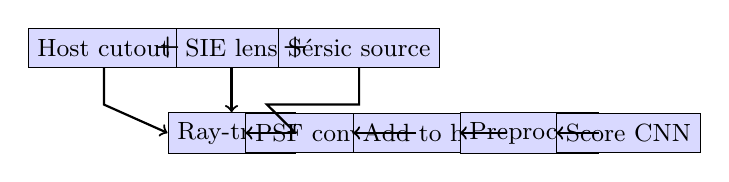
\begin{tikzpicture}[scale=0.9,
    box/.style={rectangle, draw, fill=blue!15, minimum height=0.5cm, minimum width=1.1cm, font=\small}
]
    % Row 1: Inputs
    \node[box] (host) at (0,1.2) {Host cutout};
    \node[box] (sie) at (1.8,1.2) {SIE lens};
    \node[box] (sersic) at (3.6,1.2) {S\'ersic source};
    \node at (0.9,1.2) {\textbf{+}};
    \node at (2.7,1.2) {\textbf{+}};
    
    % Row 2: Process
    \node[box] (raytrace) at (1.8,0) {Ray-trace};
    \node[box] (psf) at (3.2,0) {PSF convolve};
    \node[box] (add) at (4.6,0) {Add to host};
    \node[box] (preproc) at (6.0,0) {Preprocess};
    \node[box] (cnn) at (7.4,0) {Score CNN};
    
    % Arrows from inputs to raytrace
    \draw[->, thick] (host.south) -- (0,0.4) -- (raytrace.west);
    \draw[->, thick] (sie.south) -- (raytrace.north);
    \draw[->, thick] (sersic.south) -- (3.6,0.4) -- (2.3,0.4) -- (raytrace.east);
    
    % Arrows through pipeline
    \draw[->, thick] (raytrace) -- (psf);
    \draw[->, thick] (psf) -- (add);
    \draw[->, thick] (add) -- (preproc);
    \draw[->, thick] (preproc) -- (cnn);
\end{tikzpicture}
\caption{The injection pipeline. We combine a host cutout, an SIE lens model, and a S\'ersic source. Ray-tracing produces the lensed arc; we convolve with the PSF, add to the host in nanomaggy space, preprocess, and score with the CNN.}
\end{figure}

\subsection{Summary}

The injection pipeline produces synthetic lensed arcs using an SIE lens and a S\'ersic source. Ray-tracing, PSF convolution, and flux calibration create realistic-looking arcs in image space. We add them to real host cutouts before preprocessing and pass the result through our CNN. The pipeline is standard in the field---the same general approach used by Collett \& Cunnington and others. The question our paper asks is: do these parametric injections produce the same detection statistics as real lenses? The answer, as we will see, is no.

\bigskip
\noindent\textit{In summary: The injection pipeline combines an SIE lens, a S\'ersic source, and ray-tracing to generate synthetic lensed arcs. We convolve with a survey-matched PSF, add to real host cutouts in nanomaggy space, preprocess, and score with the CNN. S\'ersic sources are smooth and lack the internal structure of real lensed galaxies.}

\newpage
\section{Chapter 9: Results---The Gap}

This chapter presents the main results of our paper: how well the CNN finds real lenses, how well it finds our synthetic injections, and--- crucially---the large gap between the two. We then describe the key diagnostic that reveals why: the linear probe experiment.

\subsection{Real Lens Performance}

On the 112 Tier-A validation lenses, our CNN achieves \textbf{89.3\% recall} at a detection threshold of $p > 0.3$. That means we correctly identify 100 out of 112 spectroscopically confirmed lenses (100/112 $\approx$ 0.893). The 95\% Wilson confidence interval is [82.6\%, 94.0\%]: we are 95\% confident the true recall lies in that range.

\textbf{Twelve lenses are missed} at this threshold. Understanding why---host morphology, Einstein radius, depth, seeing---is the subject of ongoing analysis. For the lenses we do find, the median CNN score is \textbf{0.995}: they cluster at the very high end of the score distribution. The model is confident about real lenses.

\subsection{Injection Completeness}

When we run our injection-recovery experiment over the full parameter grid (Einstein radius 0.5--3.0 arcsec, source magnitude 23--26, varying PSF and depth), we inject 110,000 synthetic lenses. At $p > 0.3$, only \textbf{5.18\%} are detected---5,697 out of 110,000. This is the \textbf{marginal completeness}: the fraction of all injections, averaged over the grid, that the CNN finds.

Most injections in this grid are faint. Source magnitudes 23--26 produce lensed arcs that are often at the limit of detectability. It is no surprise that the overall detection rate is low. The grid is dominated by hard configurations. So the raw comparison---89.3\% real recall vs.\ 5.18\% injection completeness---is not entirely fair. The injection grid includes many genuinely difficult cases that no method would find.

\subsection{The Brightness-Matched Comparison}

To make a fairer comparison, we restrict to \textbf{bright injections}: source magnitude 18--22, which produce lensed arcs at approximately magnitude 16--21 (brighter than most grid injections). We also restrict to low $\beta_{\mathrm{frac}}$ so the arcs are prominent.

Even with these favorable conditions, detection rates are only \textbf{29--39\%}---still a factor of 2--3 below the 89.3\% Tier-A recall. So the gap is not just due to the inclusion of faint injections. When we make injections as bright as (or brighter than) typical confirmed lenses, the CNN still misses most of them. Something else is going on.

\subsection{The Linear Probe: The Paper's Key Diagnostic}

The \textbf{linear probe experiment} is the central diagnostic that reveals the nature of the gap.

Here is what we did:
\begin{enumerate}
    \item We extracted the \textbf{1280-dimensional embedding vector} from the CNN's \textbf{penultimate layer} (the layer right before the final classification head) for each of:
    \begin{itemize}
        \item 112 real Tier-A lenses
        \item 500 bright injections (magnitude 19, low $\beta_{\mathrm{frac}}$)
        \item 500 negatives
    \end{itemize}
    \item We trained a \textbf{logistic regression} (a linear classifier) to separate \emph{real lenses} from \emph{injection embeddings}. This is the ``linear probe'': we are probing what the CNN has learned by asking whether a simple linear boundary can separate the two groups in the CNN's feature space.
    \item We used \textbf{5-fold cross-validation}: we split the data into 5 folds, trained on 4 and tested on 1, rotating so every fold was tested once. We report the mean AUC and its standard deviation across folds.
\end{enumerate}

\textbf{Result:} The linear probe achieves \textbf{AUC = 0.997 $\pm$ 0.003}. Near-perfect separation. In the CNN's learned feature space, real lenses and injections live in \emph{completely different regions}. A straight hyperplane can almost perfectly classify them. The CNN ``sees'' something fundamentally different about real lenses versus our parametric injections. It is not a matter of brightness---we matched that. It is a matter of \textbf{morphology}: the spatial structure, texture, and substructure of the arcs. Real lenses have it; our S\'ersic injections do not.

\subsection{The Tier-A vs.\ Tier-B Control Probe}

We performed a control experiment to ask: how much of the separation could be due to \textbf{host galaxy} differences rather than arc morphology? Real Tier-A lenses sit on specific types of host galaxies (massive ellipticals with strong lensing cross-sections). Our injection hosts are random non-lenses from the catalog. Maybe the CNN is partly responding to the host, not just the arc.

To test this, we trained a linear probe to separate \textbf{Tier-A} (spectroscopically confirmed) from \textbf{Tier-B} (visual candidates). Both are real lenses on real hosts. The only difference is confirmation status---Tier-A are proven, Tier-B may include some impostors. This probe achieves \textbf{AUC = 0.778 $\pm$ 0.062}.

The CNN can somewhat distinguish confirmed lenses from candidates. But 0.778 is far below 0.997. The gap between real lenses and injections (0.997) is much larger than the gap between two types of real lenses (0.778). This suggests that \textbf{injection-specific features}---the smooth S\'ersic morphology---contribute substantial separation beyond any host-galaxy effect.

\subsection{The Bounding Argument}

We can bound the true ``morphology-only'' contribution to the AUC:
\begin{itemize}
    \item \textbf{Lower bound (0.778):} Tier-A vs.\ Tier-B. Both use real lenses; only confirmation status differs. Host galaxies are similar. This gives a floor for how much the CNN distinguishes lens types on real hosts.
    \item \textbf{Upper bound (0.997):} Tier-A vs.\ injections. Includes both morphology differences (smooth vs.\ real arcs) \emph{and} host differences (lens-type hosts vs.\ random negatives).
\end{itemize}

The true morphology-only AUC lies somewhere between 0.778 and 0.997. The large gap (0.997 vs.\ 0.778) means that injection-specific features contribute substantial separation beyond host effects alone. The parametric arcs look wrong to the CNN in a way that goes beyond which galaxy they are placed on.

\subsection{Fr\'echet Distances Layer by Layer}

To see \emph{where} in the network the difference emerges, we computed \textbf{Fr\'echet distances} between the real-lens and injection embedding distributions at successive layers:
\begin{itemize}
    \item \textbf{Block 0} (24 dimensions): 0.14
    \item \textbf{Block 1}: 1.45
    \item \textbf{Block 2} (48 dimensions): 10.9
    \item \textbf{Block 3} (64 dimensions): 47.2
\end{itemize}

The distance grows by a factor of \textbf{330} from the earliest to the mid-level layers. At block 0, the distributions are similar (distance 0.14)---low-level pixel statistics are comparable. The difference explodes in the learned mid-level features: texture, curvature, shape. This confirms that the gap is not merely a matter of raw pixel values. The CNN has learned representations that discriminate real from parametric arcs in its internal, abstract feature space. The barrier is morphological, encoded in the layers that build up arc-like structure.

\subsection{Visual Summaries}

Our paper includes several figures that illustrate these results. See the main paper or the companion figures for the full visualizations.

\textbf{UMAP visualization} (\texttt{fig2\_umap.pdf}): A 2D projection of the 1280-dimensional embeddings. Real lenses (gold) cluster in one region; injections (blue) in another; negatives (grey) elsewhere. The separation is visually striking.

\textbf{Score distributions}: Histograms of CNN scores. Real lenses peak near $p = 1$; injections spread around $p \approx 0.19$; negatives cluster near $p = 0$. The distributions barely overlap. See \texttt{fig3\_scores.pdf}.

\textbf{Comparison cutouts}: Side-by-side examples of 8 real lenses and 8 injections. The visual difference---real arcs with knots and structure versus smooth parametric arcs---is evident even to the eye. See \texttt{fig5\_comparison.pdf}.

\subsection{What the Gap Means}

The 84-percentage-point gap (89.3\% real recall vs.\ 5.18\% marginal injection completeness) is partly explained by the injection grid including many faint, hard configurations. But even brightness-matched injections are detected at only 29--39\%. The linear probe shows that in the CNN's feature space, real lenses and parametric injections are trivially separable (AUC 0.997). The CNN has learned to recognize something about real lens morphology that our smooth S\'ersic injections lack. Completeness maps built from these injections are \emph{lower bounds}: they tell us the CNN can find at least this many parametric lenses, but they may underestimate completeness for real lenses with richer morphology. Closing the gap---making injections that look like real lenses to the CNN---remains an open challenge. The next chapter explores one attempt: adding Poisson noise to the arcs.

\bigskip
\noindent\textit{In summary: The CNN achieves 89.3\% recall on real Tier-A lenses but only 5.18\% marginal completeness on parametric injections. Brightness-matched injections reach 29--39\%. The linear probe (AUC 0.997) shows that real lenses and injections occupy different regions of the CNN's feature space. The Tier-A vs.\ Tier-B control (AUC 0.778) bounds the host contribution; the large gap indicates injection-specific morphological mismatch. Fr\'echet distances grow 330$\times$ from early to mid-level layers, confirming the barrier is in learned features. The parametric completeness maps are lower bounds; real lenses may be more detectable than these injections suggest.}
